\chapter{Construcción de un Metamodelo}

Un metamodelo se define como un \textbf{modelo del modelo}, o un modelo sustituto (también conocido en inglés como \textit{surrogate model}), orientado a reemplazar  simulaciones por modelos que busquen capturar la naturaleza de estas mismas, y que sean computacionalmente fáciles de evaluar. Los metamodelos se utilizan en la ingeniería como herramientas para el estudio de sistemas en los que la ejecución de experimentos es limitada o muy costosa, lo cual es especialmente valioso en problemas de optimización \cite{jin2011}, aunque sus aplicaciones son variadas, como en el análisis de sistemas, diseño en ingeniería, análisis de sensibilidad y modelado de sistemas con incertidumbre \cite{forrester2008}. Algunos de los metamodelos comúnmente usados en problemas de optimización son los polinomios, las redes neuronales, los modelos Kriging y las máquinas de soporte vectorial \cite{koziel2013}.

La construcción de un metamodelo se realiza a partir de varias etapas relacionadas con diferentes áreas. En el apéndice B se encuentra una descripcion detallada de estas etapas así como de la terminología utilizada durante el proceso.

\section{Metodología}
El objetivo general en esta etapa del proyecto fue construir un metamodelo $\hat{f}(\mathbf{x})$ que capturara la relación entre las variables de diseño $\mathbf{x}$ y la función objetivo definida en el capítulo anterior:
\begin{equation*}
f(\mathbf{x}) = \frac{F_x^2}{P_j}
\end{equation*}

De esta forma, una vez se ha construido un metamodelo confiable, este puede reemplazar las simulaciones obtenidas por medio del FEM en la etapa de optimización, reduciendo el costo computacional del algoritmo que realiza el proceso. Los recursos destinados para la construcción del metamodelo se fijaron en 2000 simulaciones en total, que en el computador en el que se realizaron tomaron 48 horas ininterrumpidas.

Para la construcción del metamodelo se utilizaron tres herramientas de software:
\begin{enumerate}
\item COMSOL Multiphysics 4.3: Por medio del método de elementos finitos, fue utilizado en la construcción del metamodelo para obtener los resultados de los experimentos especificados durante el diseño inicial y los diseños secuenciales, que requieren encontrar el valor de la función objetivo para diferentes valores de las variables de diseño.
\item Toolbox SUMO (\textit{SUrrogate MOdeling}): es un toolbox desarrollado para MATLAB que, citando la información en su página web \cite{sumoabout}, resuelve el problema de "generar automáticamente un metamodelo altamente preciso para un código de simulación computacionalmente costoso, requiriendo tan pocos datos y interacción con el usuario como sea posible". Este toolbox contiene todas las herramientas para obtener el diseño inicial, entrenar el metamodelo, evaluar el error con diferentes métricas, y producir los diseños secuenciales \cite{gorissen2010b}.
\item MATLAB: Usado como interfaz entre COMSOL y SUMO.
\end{enumerate}

Los métodos específicos seleccionados para las etapas de construcción del metamodelo descritas anteriormente se especifican a continuación.

\subsection{Experimentos preliminares y filtrado de variables}
El primer paso para el desarrollo del metamodelo consiste en identificar las variables que tienen una mayor influencia en el valor de la función objetivo. Con este fin, inicialmente se realizaron simulaciones ajustando las variables de diseño dentro de los intervalos definidos por las restricciones del problema.

Debido a que el número de variables es relativamente bajo ($n < 10$) y que las variables se escogieron con base en el conocimiento del sistema, se decidió realizar el filtrado de variables por medio del coeficiente de correlación R$^2$. Para esta etapa se destinaron 1000 simulaciones, y con estos datos posteriormente se encontró el coeficiente R$^2$ entre cada una de las variables de diseño y la función objetivo. Los resultados se ilustran en la Fig. \ref{fig:corrcoeff}.

\begin{figure}[t]
\centering
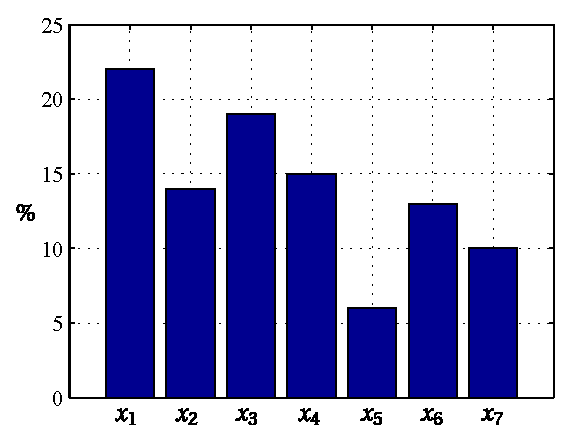
\includegraphics[scale=0.9]{../img/Construccion_de_un_Metamodelo/corrcoeff2.eps}
\caption{Coeficientes de correlación.}
\label{fig:corrcoeff}
\end{figure}

En promedio, los coeficientes de correlación están alrededor del 15\%, sin embargo es notoria la baja correlación entre la variable $x_5$ (la altura posterior del núcleo) y la función objetivo. Por esta razón, se decidió mantenerla fija, asignándole el valor obtenido durante el proceso de diseño inicial y eliminar este parámetro como variable de diseño, reduciendo la dimensionalidad a $n=6$. Así, se redefinieron las variables de diseño como sigue:
\begin{itemize}
\item $x_1$: Paso polar
\item $x_2$: Ancho del motor
\item $x_3$: Razón ancho de ranura - paso de ranura
\item $x_4$: Alto de ranura
\item $x_5$: Corriente de fase
\item $x_6$: Número de vueltas por bobina
\end{itemize}

\subsection{Diseño inicial}
Teniendo en cuenta que el diseño factorial completo, aunque simple, es poco eficiente computacionalmente, se decidió utilizar un diseño de hipercubo latino, debido a que es un proceso que SUMO realiza de manera automática y es aplicable de acuerdo al número de dimensiones del problema.

\subsection{Métrica de error y estructura del metamodelo}
Existen diversas métricas de error, tanto absolutas como relativas, que pueden ser de utilidad para la evaluación del metamodelo y que pueden producir resultados, como el error euclidiano promedio, el error geométrico promedio y el error cuadrático relativo, entre otros, que pueden producir resultados satisfactorios, o poco eficientes si no se seleccionan adecuadamente \cite{gorissen2010}.
En esta etapa se realizó un análisis de los valores de la función objetivo en el conjunto de entrenamiento. Un histograma para los valores de la función objetivo obtenido a partir de varios valores para las variables de diseño se muestra en la Fig. \ref{fig:fobjhist}. En esta el valor de la función objetivo para el diseño del MLR inicial se resalta con una línea roja.
\begin{figure}[t]
\centering
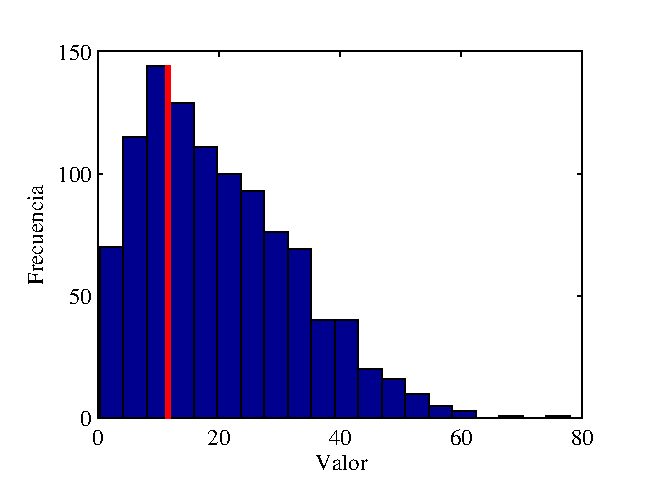
\includegraphics[scale=0.9]{../img/Construccion_de_un_Metamodelo/fobjhist.eps}
\caption{Histograma de los valores de la función objetivo.}
\label{fig:fobjhist}
\end{figure}
De este histograma se observa que existe una predominancia alrededor del valor objetivo del diseño inicial del MLR, y los valores decaen a ambos lados, sin saltos pronunciados a ambos lados de este valor, hasta un rango de 80, por lo que, siguiendo las sugerencias expuestas en \cite{gorissen2010}, se prefirió utilizar una métrica de error absoluta. De estas métricas se seleccionó el error euclidiano promedio (AEE, de las siglas en inglés de \textit{Average Euclidian Error}), debido a que, aunque puede ser una medida ``pesimista'' (errores grandes son penalizados en exceso, y errores pequeños son casi ignorados), es menos pesimista que otras métricas como el RMSE. Además, es una medida verdadera de la distancia aritmética entre el valor real y el valor estimado, lo cual presenta una ventaja a la hora de entender los valores obtenidos para esta métrica a partir de determinado metamodelo \cite{rong2006}.

Con respecto a la estructura del metamodelo, se decidió experimentar con cuatro posibles opciones: un modelo racional (superficie polinomial), una función de base radial (RBF), una máquina de soporte vectorial (SVM) y una red neuronal artificial (ANN). Los métodos de optimización utilizados para el entrenamiento fueron el ascenso de colinas (también conocido como \textit{hill climbing}), el algoritmo genético y la optimización por enjambre de partículas. Estos modelos y métodos se seleccionaron debido a que se contaba con experiencia previa en el uso de los mismos.

\subsection{Diseño secuencial}
Debido a que SUMO contiene la funcionalidad necesaria para implementar diseños secuenciales que combinan explotación y exploración, se decidió trabajar con el algoritmo LOLA-Voronoi para este fin, teniendo en cuenta de igual forma que es el único algoritmo de diseño secuencial implementado en SUMO con soporte para variables con restricciones (el cual es el caso para el sistema tratado).

\section{Resultados}
Después de entrenar cada uno de los metamodelos utilizando diferentes métodos, se seleccionaron aquellos que presentaron el menor AEE. El mejor metamodelo de tipo RBF se obtuvo por medio del ascenso de colinas, el racional por medio del algoritmo genético, el tipo SVM por medio de optimización por enjambre de partículas y la ANN por medio del algoritmo genético. Es evidente que el mejor metamodelo obtenido corresponde a la red neuronal, que alcanzó valores del AEE de alrededor de un orden de magnitud menos que los demás metamodelos, a pesar de que fue el que más tiempo tomó durante el entrenamiento para llegar al valor final del AEE (30 horas, en comparación con los demás modelos, que tomaron dos o hasta tres veces menos, en el computador en el que se realizó el entrenamiento).

Tal como se describió anteriormente, el proceso de construcción del metamodelo es iterativo, realizándose el entrenamiento del mismo con un número de muestras predeterminado hasta que se cumplen los criterios de entrenamiento, a lo que sigue el diseño secuencial y se repite hasta que se agotan los recursos. Durante cada iteración en la que se obtenía un mejor AEE, se obtuvo el valor correspondiente para cada modelo por medio de validación cruzada, como se muestra en la Fig. \ref{fig:bestprofiler}. Es claro como desde el inicio de la construcción del metamodelo, la ANN inició con un valor bajo del AEE en comparación con los demás, llegando a valores aún más bajos al final del proceso.

La red neuronal obtenida como el mejor metamodelo posee dos capas ocultas, cada una con 13 y 14 neuronas, respectivamente, y debido a que puede operar con matrices donde cada columna es un vector de diseño, su implementación produce resultados que efectivamente reducen el costo computacional del modelo original: mientras con el método FEM se evaluaron 1000 experimentos en 24 horas, la red neuronal permitió evaluar el mismo número en 6 milisegundos.

\begin{figure}[t]
\centering
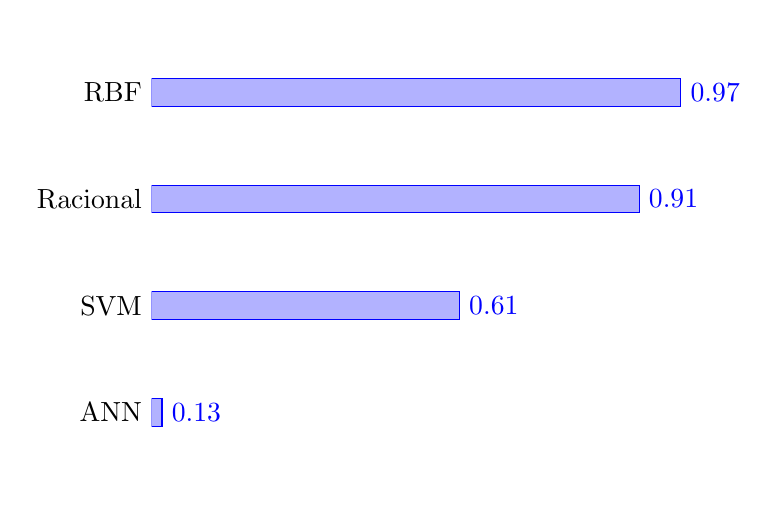
\begin{tikzpicture}
  \begin{axis}[
    xbar,
    y axis line style = { opacity = 0 },
    axis x line       = none,
    tickwidth         = 0pt,
    enlarge y limits  = 0.2,
    enlarge x limits  = 0.02,
    symbolic y coords = {ANN,SVM,Racional,RBF},
    nodes near coords,
  ]
  \addplot coordinates {(0.127,ANN)(0.612,SVM)(0.905,Racional)(0.973,RBF)};
  \end{axis}
\end{tikzpicture}
\caption{Mejores valores del AEE obtenidos.}
\label{fig:bestaee}
\end{figure}

\begin{figure}[t]
\centering
\includegraphics[scale=0.9]{../img/Construccion_de_un_Metamodelo/bestprofiler.eps}
\caption{Error de validación cruzada del mejor metamodelo.}
\label{fig:bestprofiler}
\end{figure}

\section{Conclusiones}
Los resultados mostrados a lo largo del capítulo indican que los esfuerzos invertidos en la construcción de un metamodelo fueron útiles debido a que se logró reducir la dimensionalidad del problema y se obtuvo una red neuronal como metamodelo para la función objetivo del problema de optimización definida en el capítulo anterior.  

En \cite{farmaga2011} se encuentra una medida de la complejidad computacional del FEM, que en el peor de los casos puede ser exponencial. En este sentido, se concluye que el uso del metamodelo es un método que permite reducir los efectos de la maldición de la dimensionalidad sobre problemas de optimización con varias variables de diseño, con respecto a la aplicación directa del FEM, debido a que su operación se basa en operaciones con matrices que son ejecutadas de manera eficiente por el software utilizado.

\bibliographystyle{ieeetr}
\bibliography{../refs}